%\documentclass[aps,twocolumn,secnumarabic,balancelastpage,amsmath,amssymb,nofootinbib,floatfix]{revtex4-1}

\documentclass{report}

\usepackage[colorlinks=true,linkcolor=blue]{hyperref}

% \usepackage{mathexam}
% \usepackage{booktabs}

% \usepackage{a4wide}
\usepackage[utf8]{inputenc}
\usepackage{amsmath}
\usepackage{amsfonts}
\usepackage{amssymb}
\usepackage{mathtools}
\usepackage[brazil]{babel}
%quebra de linha do sumário
%\usepackage[breaklinks=true]{hyperref}
%\usepackage{braket}
\usepackage{minitoc}
\usepackage{wrapfig}
\usepackage{subfigure}
\usepackage{setspace}
\usepackage{underscore}
\usepackage{indentfirst}
\usepackage{physics}

\usepackage{accents}

\usepackage{blindtext}

\usepackage{graphicx}
\usepackage{tikz}
\usetikzlibrary{shapes,arrows}

\usepackage{listings}
\usepackage{color}

\definecolor{mygreen}{rgb}{0,0.6,0}
\definecolor{mygray}{rgb}{0.85,0.85,0.85}
\definecolor{mymauve}{rgb}{1,0.502,0}
\definecolor{numGray}{rgb}{0.3,0.3,0.3}

\lstset{language=C,
  backgroundcolor=\color{mygray},   % choose the background color; you must add \usepackage{color} or \usepackage{xcolor}; should come as last argument
  basicstyle=\footnotesize,        % the size of the fonts that are used for the code
  breakatwhitespace=false,         % sets if automatic breaks should only happen at whitespace
  breaklines=true,                 % sets automatic line breaking
  captionpos=b,                    % sets the caption-position to bottom
  commentstyle=\color{mygreen},    % comment style
  deletekeywords={...},            % if you want to delete keywords from the given language
  escapeinside={\%*}{*)},          % if you want to add LaTeX within your code
  extendedchars=true,              % lets you use non-ASCII characters; for 8-bits encodings only, does not work with UTF-8
  frame=single,	                   % adds a frame around the code
  keepspaces=true,                 % keeps spaces in text, useful for keeping indentation of code (possibly needs columns=flexible)
  keywordstyle=\color{blue},       % keyword style
  language=C,                 % the language of the code
  morekeywords={*,...},            % if you want to add more keywords to the set
  numbers=left,                    % where to put the line-numbers; possible values are (none, left, right)
  numbersep=5pt,                   % how far the line-numbers are from the code
  numberstyle=\tiny\color{numGray}, % the style that is used for the line-numbers
  rulecolor=\color{black},         % if not set, the frame-color may be changed on line-breaks within not-black text (e.g. comments (green here))
  showspaces=false,                % show spaces everywhere adding particular underscores; it overrides 'showstringspaces'
  showstringspaces=false,          % underline spaces within strings only
  showtabs=false,                  % show tabs within strings adding particular underscores
  stepnumber=1,                    % the step between two line-numbers. If it's 1, each line will be numbered
  stringstyle=\color{mymauve},     % string literal style
  tabsize=2,	                   % sets default tabsize to 2 spaces
  title=\lstname                   % show the filename of files included with \lstinputlisting; also try caption instead of title
}




\onehalfspacing


\newcommand*{\dt}[1]{%
  \accentset{\mbox{\large\bfseries .}}{#1}}
\newcommand*{\ddt}[1]{%
  \accentset{\mbox{\large\bfseries .\hspace{-0.25ex}.}}{#1}}
\newcommand*{\dddt}[1]{%
  \accentset{\mbox{\large\bfseries .\hspace{-0.25ex}.\hspace{-.20ex}}}{#1}}
\newcommand*{\dnt}[2][4]{\dt{#2}^{\tiny(#1)}}
\newcommand{\esimo}{-\text{ésimo}}
\newcommand{\esima}{-\text{ésima}}

\makeatletter
\newcommand*{\gnuplotinput}[2][1.0]{%
  \begingroup
  \let\@gnplt@input@includegraphics=\includegraphics
  \def\includegraphics##1{\@gnplt@input@includegraphics[scale=#1]{#2}}%
  \let\@gnplt@input@picture=\picture
  \def\picture{\unitlength=#1\unitlength\relax\@gnplt@input@picture}%
  \input{#2}%
  \endgroup
}
\makeatother

\newcommand{\PraticeQuestion}[2]{
  \begin{center}
    \LARGE \textbf{Física Computacional - Prática #1} \\
    \Large \textbf{Questão #2} \\
    \large Alex Enrique Crispim
  \end{center}
}


\begin{document}
  \PraticeQuestion{10}{2}

  Utilizando o programa \texttt{ising2d.f}, calculou-se, via Monte Carlo com o Algoritmo de Metropolis, o valor da magnetização média absoluta $\ev{\abs{M}}$, variando-se a temeperatura ($\beta$, equivalentemente).

  A solução de Onsager nos dá o valor da transição de fase:
  \begin{equation*}
    \beta_c = \frac{\ln(1+ \sqrt{2})}{2J} .
  \end{equation*}


  A temeperatura de transição de fase se dá em $2.269185314$ (unidades arbitrárias utilizadas no programa, isto é, $k = 1$ e $J = 1$). Variando-se $\beta$ de 0.34 até 1.0, é passamos pela transição de fase, de tal modo que devemos ver uma curva tentendo para uma descontinuidade em tal temeperatura.

  Na verdade, não se vê de fato tal descontinuidade por conta do \textit{efeito de rede finita}. Se se fizer, por outro lado, um \textit{finite size scalling}, aumentando-se $N$, de modo a determinar o valor do observável no limite termodinâmico, o resultado se aproximará da solução exata conhecida.

  Abaixo temos o gráfico obtido, em comparação com a solução exata, em vermelho.

  \begin{figure}[h]
    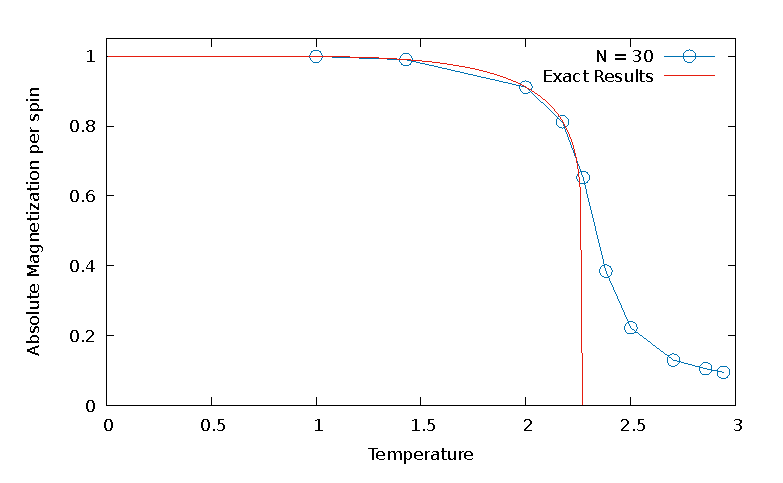
\includegraphics[scale = 1.0]{Mabs.eps}
  \end{figure}

  \newpage
  Da figura, vê-se que acima da temperatura de transição, o valor do observável tende para zero, mas se desvia do teórico esperado. Abaixo da temperatura crítica, por outro lado, temos uma grande concordância com o resultado teórico.

  Isso nos diz que o resultado encontrado nos permite inferir a cerca da solução teórica, corroborando para a mesma.

  Como veremos na questão 4, o resultado numérico se torna mais fiél ao resultado exato quando $N$ aumenta.

\end{document}
